\section{Travaux réalisés en Java, le \textit{Text Mining} et le \textit{Natural Language Processing} avec la bibliothèque de Stanford}
\label{sec:travaux_realises_en_java}
    \subsection{Présentation de mon environnement de travail}
        Dans C-Radar tout les traitements de type \og computing \fg (calcul) sont réalisés en Python (cf partie \ref{subsub:archi_tech}). De ce fait, créer une application permettant de classifier les signaux, devrait être fait en Python sous la forme d'un plugin. Ayant fait le choix de commencer mes recherches en Java, il a fallu m'initialiser un environnement de travail un peu différent de l'environnement de travail Python.

        \paragraph{Spring et MongoDB :}
            Loïc Petit m'a créé une application Spring de base permettant de me connecter en local à une base de données Mongo. Ce projet Spring est géré avec Maven. L'application me fournit un environnement de travail dans lequel construire le classifieur à partir des signaux validés récupérés depuis une base de données Mongo. Cette base de données contient mon ensemble de signaux permettant de construire et tester mon classifieur. Les 1426 signaux validés y sont stocké ainsi que 350.000 autres signaux non validés (voir le dernier paragraphe de la partie \ref{sec:etat_bd}).\\

        Voici comment les signaux sont stockés dans Mongo :
\begin{verbatim}
{
    "id" : "TWITTER:agencenetdesign:329129810423083009",
    "content" : "Salon eCom Genève : l'équipe ND est en place au stand E1 \:) #ecomSITB http://t.co/YtsEs6rcDR",
    "publicationDate" : ISODate(2013-04-30T07:07:16Z),
    "sourceId" : "TWITTER:agencenetdesign",
    "source" : {
        "type" : "TWITTER",
        "resourceId" : "agencenetdesign"
    },
    "externalSignalId" : 329129810423083009,
    "validated" : false,
    "validatedTags" : [ ],
    "tags" : [
        "EVENT"
    ],
    "url" : "http://twitter.com/agencenetdesign/status/329129810423083009"
}
\end{verbatim}

        Le signal comporte :
        \begin{itemize}
            \item un identifieur unique \textit{id} ;
            \item un contenu \textit{content} ;
            \item une date de publication \textit{publicationDate} ;
            \item l'identifieur de la source \textit{sourceId} ;
            \item la source \textit{source} composé :
            \begin{itemize}
                \item du type de réseau dont provient le signal \textit{type} ;
                \item de l'identifieur du publieur dans ce réseau \textit{resourceId} ;
            \end{itemize}
            \item un identifeur externe \textit{externalSignalId} ;
            \item un booléen spécifiant si le signal a été manuellement validé ou non \textit{validated} ;
            \item la liste des tags s'il a été validé \textit{validatedTags}, la liste des tags potentiels (trouvés par le classifieur) \textit{tags} ;
            \item l'url là où a été publié le signal \textit{url}.
        \end{itemize}

        \paragraph{Formation Spring et Mongo :}
            Je me suis rapidement formé à Spring et Mongo pour pouvoir interfacer ces deux composants ensemble. Pour cela, j'ai suivi les tutoriels de Spring disponibles sur \href{https://spring.io/guides/gs/accessing-data-mongodb/}{https://spring.io/guides/gs/accessing-data-mongodb/}.\\
            Grâce aux tutoriels, j'ai appris à créer mes premiers points d'API permettant de faire des requêtes dans Mongo. Ces requêtes sont relativement basiques : récupérer tout les signaux sous forme de liste, récupérer uniquement les signaux validés (également sous forme de liste), savoir combien de signaux sont stockés dans ma base, etc. La documentation de Mongo disponible sur \href{https://docs.mongodb.org/manual/}{https://docs.mongodb.org/manual/} m'a également bien aidé. Les concepts de base de Mongo ne sont pas très compliqués à comprendre quand on a des notions de base de données.\\

        Dès que j'ai été capable de faire ce type de requêtes auprès de ma base de données, il fallait me concentrer sur le traitement des signaux, et donc construire un classifieur. C'est à ce moment que je me suis intéressé à la bibliothèque de Stanford.

        \subsection{La bibliothèque : Stanford Natural Language Processing}
            Samuel Charron m'a conseillé de me former en \textit{Text Mining} et en \textit{Natural Language Processing} au travers de cette bibliothèque implémentée en Java. Celle-ci propose un ensemble d'outils pour le traitement automatique de la langue anglaise, chinoise et espagnole.

            \subsubsection{Les cours de l'université de Stanford sur le \textit{Natural Language Processing}}
                Ces cours accessibles librement sur Internet, m'ont permis de découvrir de nombreux concepts (expliqués ci-après et en partie \ref{ssec:premiere_mise_en_appli}) :
                \begin{itemize}
                    \item Le modèle du \textit{bag of words} ;
                    \item Le modèle \textit{maximum entropy} ;
                    \item Les prétraitements comme la lemmatisation.
                \end{itemize}
                Ces cours proviennent du livre \textit{Introduction to Information Retrieval}\autocite{ir_web}.\\

                En parallèle, j'ai visionné sur coursera les vidéos que cette même université avait diffusé suite à un MOOC sur le \textit{Natural Language Processing}. Grâce à ces cours, j'ai pris conscience de l'importance de bien choisir son modèle de classifieur. De plus, j'ai également compris l'intérêt des prétraitements, permettant de normaliser et formater les données textuelles afin d'augmenter les performances et la capacité de généralisation du classifieur.\\

                Durant ma formation au \textit{Natural Language Processing}, j'ai également lu les livres \textit{Natural Language Processing with Python}\autocite{nlp_p} et \textit{Python 3 Text Processing with NLTK 3 Cookbook}\autocite{nltk}, ainsi que les pages internets \textit{Introduction to Information Retrieval}\autocite{ir_web}.

            \subsubsection{Stanford POS Tagger (Part-Of-Speech) :}
                Le \textit{POS Tagger} permet de savoir la fonction grammaticale de chaque mot d'une phrase. Celui-ci fonctionne aussi pour le français.

                \paragraph{Exemple :}
                    Entrée \og Gustave is the firstname of a very famous french architect.\fg\\
                    Sortie :
\begin{lstlisting}
K$\overbrace{Gustave}^{\highlight[cyan]{NNP}} \overbrace{is}^{\highlight[green]{VBZ}} \overbrace{the}^{\highlight[magenta]{DT}} \overbrace{firstname}^{\highlight[cyan]{NN}} \overbrace{of}^{\highlight[orange]{IN}} \overbrace{a}^{\highlight[magenta]{DT}} \overbrace{very}^{\highlight[yellow]{RB}} \overbrace{famous}^{\highlight[yellow]{JJ}} \overbrace{french}^{\highlight[yellow]{JJ}} \overbrace{architect}^{\highlight[cyan]{NN}}\overbrace{.}^{\highlight[gray]{.}}$W
\end{lstlisting}
                \textit{$\highlight[cyan]{NNP}$} signifie qu'il s'agit d'un nom propre singulier (\textit{noun, proper, singular}), \textit{$\highlight[green]{VBZ}$} signifie qu'il s'agit d'un verbe à la 3ème personne du singulier au présent (\textit{verb, present tense, 3rd person singular}), \textit{$\highlight[magenta]{DT}$} signifie qu'il s'agit d'un déterminant (\textit{determiner}), \textit{$\highlight[cyan]{NN}$} signifie qu'il s'agit d'un nom commun singulier (\textit{noun, common, singular}), \textit{$\highlight[orange]{IN}$} signifie qu'il s'agit d'une préposition ou d'une conjonction de subordination (\textit{preposition or conjunction, subordinating}), \textit{$\highlight[yellow]{RB}$} signifie qu'il s'agit d'un adverbe (\textit{adverb}) et \textit{$\highlight[yellow]{JJ}$} signifie qu'il s'agit d'un adjectif (\textit{adjective}).

            \subsubsection{Stanford Parser :}
                Le \textit{Parser} permet de connaître la structure grammaticale d'une phrase, à savoir quel(s) groupe(s) de mots forme(nt) le sujet, le verbe et le complément. Cet outils est une sur-couche du \textit{POS Tagger} puisqu'il réutilise son résultat.

                \paragraph{Exemple :}
                Entrée \og My internship was a rewarding experience.\fg\\
                Sortie :
\begin{lstlisting}
K(\textcolor{blue}{ROOT}W
  K(\textcolor{blue}{S}W
    K(\textcolor{cyan}{NP} (\textcolor{pink}{PRP}\$ My) (\textcolor{cyan}{NN} internship))W
    K(\textcolor{green}{VP} (\textcolor{green}{VBD} was)W
      K(\textcolor{cyan}{NP} (\textcolor{magenta}{DT} a) (\textcolor{yellow}{JJ} rewarding) (\textcolor{cyan}{NN} experience))W
    K(\textcolor{gray}{.} .)))W
\end{lstlisting}

            \subsubsection{Stanford Named Entity Recognizer :}
                Le \textit{Named Entity Recognizer} permet d'identifier les groupes de mots qui sont des noms de personne, d'entreprises, de gènes, etc.

                \paragraph{Exemple :}
                Entrée \og François Bancilhon is the CEO of Data Publica, a Startup located in Paris.\fg\\
                Sortie :
\begin{lstlisting}
K$\highlight[magenta]{François}$W K$\highlight[magenta]{Bancilhon}$W is the CEO of K$\highlight[orange]{Data}$W K$\highlight[orange]{Publica}$W, a Startup located in K$\highlight[violet]{Paris}$W.
\end{lstlisting}
                Les mots surlignés en magenta comme $\highlight[magenta]{François}$ $\highlight[magenta]{Bancilhon}$ sont potentiellement des noms de personnes (\textit{$\highlight[magenta]{PERSON}$}). Ceux surlignés en orange comme $\highlight[orange]{Data}$ $\highlight[orange]{Publica}$ sont potentiellement des noms d'organisations (\textit{$\highlight[orange]{ORGANIZATION}$}). Enfin, les mots surlignés en violet comme $\highlight[violet]{Paris}$ sont potentiellement des noms de lieux (\textit{$\highlight[violet]{LOCATION}$}).

            \subsubsection{Stanford Classifier :}
                Le \textit{Classifier} permet de construire un classifieur automatique pour la catégorisation de texte. Un classifieur \textit{maximum entropy} et un naïf bayésien sont disponibles. Cet outils propose une classe (\textit{ColumnDataClassifier}) qui permet de construire n'importe quel type de classifieur, simplement en lui fournissant un fichier de configurations, et des données d'apprentissage et de test. Le soucis de cette classe est que les données doivent se conformer à un format bien précis.

            \subsubsection{Stanford CoreNLP :}
                Le \textit{CoreNLP} permet de construire une suite de traitements automatiques (les traitements précédents) sur de l'anglais, du chinois, de l'espagnol. Un exemple de chaîne de traitement est visible en figure \ref{fig:coreNLP}. La particularité de cet outils, est qu'il permet de réutiliser les traitements précédents les uns à la suite des autres (sauf le \textit{Stanford Classifier}). De plus, il permet aussi d'appliquer des traitements supplémentaires à ceux énoncés jusque là. En effet, celui-ci permet de faire de la recherche morphologique telle que lemmatisation ou stemming. Le \textit{POS Tagger} et le \textit{Tokenizer} sont réutilisés pour ces traitements.

                %\paragraph{Fonctionnement :}
                %L'entité manipulée dans la classe \textit{StanfordCoreNLP} est le \textit{pipeline}. Le \textit{pipeline} est donc l'objet permettant de créer des chaînes de traitement. Il possède une liste de propriétés. Il suffit d'ajouter un objet appelé \textit{Annotator} aux propriétés du \textit{pipeline} pour que celui-ci réalise un traitement précis.\\
                %Par exemple, \textit{TokenizerAnnotator} est l'\textit{Annotator} permettant d'appliquer le traitement du \textit{Stanford Tokenizer} sur le texte donné en entrée.\\
                %Le fonctionnement est le suivant : Premièrement, il faut instancier un objet \textit{pipeline} et lui assigner des \textit{Annotators}. Ainsi, une série de traitements devra être réalisée lors de l'appel de sa méthode principale \textit{annotate()}. Ensuite, il n'y a plus qu'à passer une chaîne de caractère à cette méthode \textit{annotate()} pour obtenir un objet annoté en retour.

            \subsubsection{Lemmatisation et stemming :}
                La lemmatisation consiste à trouver les lemmes de chaque mots d'une phrase. Ce traitement est détaillé en partie \ref{ssubsec:travaux_globaux}. Ce traitement nécessite que la phrase soit préalablement découpée en token (les mots de la phrase) par un \textit{Tokenizer} et que chacun d'entre eux soit tagué par le \textit{POS Tagger}. Ainsi, en couplant la fonction grammaticale d'un mot avec un dictionnaire, il est possible de retrouver le lemme du mot.

                \paragraph{Exemple :}
                Entrée \og No better example than these could have been found.\fg\\
                Sortie :
\begin{lstlisting}
K$\overbrace{No}^{\highlight[yellow]{no}}\ \overbrace{better}^{\highlight[yellow]{good}}\ \overbrace{example}^{\highlight[cyan]{example}}\ \overbrace{than}^{\highlight[orange]{than}}\ \overbrace{these}^{\highlight[magenta]{this}}\ \overbrace{could}^{\highlight[green]{can}}\ \overbrace{have}^{\highlight[green]{have}}\ \overbrace{been}^{\highlight[green]{be}}\ \overbrace{found}^{\highlight[green]{find}} \overbrace{.}^{\highlight[gray]{.}}$W
\end{lstlisting}

                \paragraph{Le stemming :}
                Le stemming est un traitement assez similaire à la lemmatisation. Celui-ci consiste à trouver les stems et non les lemmes. Ce traitement est détaillé en partie \ref{ssubsec:travaux_globaux}.

                \paragraph{Exemple :}
                Entrée \og Les chevaliers chevauchent leur chevaux, le cavalier son cheval.\fg\\
                Sortie :
\begin{lstlisting}
K$\overbrace{Les}^{le}\ \overbrace{chevaliers}^{cheva}\ \overbrace{chevauchent}^{cheva}\ \overbrace{leur}^{leur}\ \overbrace{chevaux}^{cheva} \overbrace{,}^{,}\ \overbrace{le}^{le}\ \overbrace{cavalier}^{caval}\ \overbrace{son}^{son}\ \overbrace{cheval}^{cheva} \overbrace{.}^{.}$W
\end{lstlisting}

            \begin{figure}[h!]
                \centering
                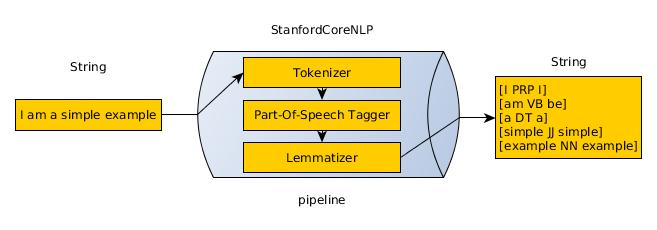
\includegraphics[width=\textwidth]{images/coreNLP.jpg}
                \caption{Trois traitements sont assignés au \textit{pipeline} (entité de la classe \textit{StanfordCoreNLP}) : \textit{Tokenization}, \textit{POS-Tagging} et \textit{Lemmatization}. En sortie, une chaîne de caractère présente le résultat de chaque traitement en colonne.}
                \label{fig:coreNLP}
            \end{figure}

            \subsubsection{Premier bilan sur la bibliothèque}
                Dans un premier temps, mon objectif est seulement de réutiliser la partie \textit{Stanford Classifier} de la bibliothèque pour créer un classifieur binaire. Celui-ci doit être capable de classifier les signaux relatifs aux offres d'emploi et de stage (soit le tag \textit{JOB}). La classe \textit{ColumnDataClassifier} va mettre d'une grande aide, même si elle exige des données dans un format particulier et qu'elle ne gère pas certain prétraitements.\\

                Des traitements comme la lemmatisation ou le stemming seront utiles, lors de la normalisation des données. Pouvoir utiliser le \textit{StanfordCoreNLP} pour normaliser et sélectionner les features utiles serait l'idéal, avant de les fournir au classifieur pour construire un modèle.

        \subsection{Première mise en pratique de la bibliothèque de Stanford}
        \label{ssec:premiere_mise_en_appli}
            \subsubsection{Première application Spring}
                J'ai construis une application réalisant les actions suivantes (visible en figure \ref{fig:classif_building} et expliquée ci-après) :
            \begin{itemize}
                \item Récupérer les signaux stockés dans Mongo sous forme de liste ;
                \item Créer un ensemble de données à partir des signaux validés manuellement ;
                \item Diviser aléatoirement cet ensemble de données en deux ensembles (un pour entraîner le classifieur et un pour le tester) tout en gardant la proportion de chaque classe dans les deux ensembles ;
                \item Entraîner un classifieur binaire naïf bayésien ;
                \item Fixer les hyper-paramètres du classifier par validation croisée pendant la phase d'apprentissage ;
                \item Évaluer la qualité du classifieur construit (l'erreur de généralisation) en calculant sa précision et son rappel sur un ensemble de données de test (qui n'ont pas \og été vu \fg jusqu'à ici par le classifieur).
            \end{itemize}

            \begin{figure}[h!]
                \centering
                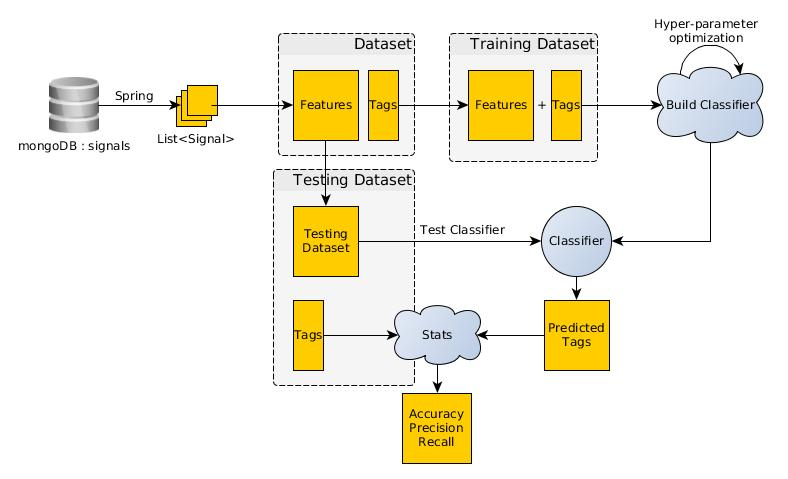
\includegraphics[width=\textwidth]{images/classifier_building.jpg}
                \caption{La construction du classifieur.}
                \label{fig:classif_building}
            \end{figure}

            \subsubsection{Le modèle de classifieur}
                Quel type de classifieur construire ? Un SVM ? Une régression logistique ? Un modèle naïf bayésien ?\\
                Dans la littérature de la classification de texte, comme la détection de spam dans les emails ou l'analyse des sentiments (savoir si un texte est critique ou élogieux), il est plutôt commun de construire des classifieurs naïf bayésien avec comme caractéristiques la fréquence des mots. Ainsi, j'ai choisi de construire un tel classifieur pour catégoriser mes signaux. (C'est également ce qu'avait fait Samuel Charron en Python.)

            \subsubsection{Construction de l'ensemble de données}
                Ensuite, s'est poser la question de comment utiliser les données labellisées pour construire un ensemble de données pour l'apprentissage et la validation. Sur ce point, j'ai choisi de construire mon ensemble de données selon le modèle du \textit{bag of words}.\\

                Dans ce modèle, un texte (une phrase ou un document) est représenté comme un sac (\textit{bag}), un ensemble de ses mots (au sens mathématique), sans se préoccuper de la grammaire ou de l'ordre des mots, mais en gardant la multiplicité. Ce modèle est communément utilisé en classification de document, quand la fréquence, l’occurrence des mots est utilisé comme caractéristique. C'est le cas du modèle naïf bayésien.\\

                Ainsi, un signal est caractérisé par la liste des occurrences des mots de son titre et son contenu.

            \paragraph{Exemple :}
                Modélisation de deux signaux à l'aide du \textit{bag of words} :
\begin{lstlisting}
K$Offre\ d'emploi\ :\ Ingénieur\ d’études\ et\ développement\ Java.$W
K$Offre\ de\ stage\ :\ Classification\ de\ signaux\ entreprises\ Java\ ou\ Python.$W
\end{lstlisting}
                À partir de ces deux signaux, une liste de mot est construite à l'aide d'un tokenizer :
\begin{verbatim}
[ "Offre", "d'", "emploi", ":", "Ingénieur", "études", "et", "développement",
  "Java", ".", "de", "stage", "Classification", "signaux", "entreprises",
  "ou", "Python" ]
\end{verbatim}
                Celle-ci contient 17 mots distincts. En utilisant son index, on peut représenter chaque signal comme un vecteur de taille 17 :
\begin{lstlisting}
K$[\ 1,\ 2,\ 1,\ 1,\ 1,\ 1,\ 1,\ 1,\ 1,\ 1,\ 0,\ 0,\ 0,\ 0,\ 0,\ 0,\ 0\ ]$W
K$[\ 1,\ 0,\ 0,\ 1,\ 0,\ 0,\ 0,\ 0,\ 1,\ 1,\ 2,\ 1,\ 1,\ 1,\ 1,\ 1,\ 1\ ]$W
\end{lstlisting}
                Chaque ième composante du vecteur représente le nombre de fois que le ième mot de la liste est présent dans le signal. Par exemple, dans le premier vecteur (représente le premier signal), les deux premières composantes sont \og 1, 2 \fg. La première composante correspond au mot \og Offre \fg qui est le premier mot de la liste, et sa valeur est \og 1 \fg car \og Offre \fg est présent une fois dans le premier signal. De la même façon, la deuxième composante correspond au mot \og d' \fg, le deuxième mot de la liste et sa valeur est \og 2 \fg car il est présent deux fois dans le signal.\\

                Quelque soit le classifieur que j'ai construis par la suite, l'ensemble de données est toujours construit suivant ce modèle. Pour mon premier classifieur binaire, les 123 signaux validés \textit{JOB} de l'ensemble des 1426 signaux validés (présentés dans le dernier paragraphe de la partie \ref{sec:etat_bd}), forment la classe \textit{JOB} contre le reste.\\

                Enfin, le seul pré-traitement des données mis en place est le fait de garder les éléments du \textit{bag of words} apparaissant au moins cinq fois. Ceci afin de supprimer les mots rares qui n'apportent pas d'informations, quand on fait de la classification textuelle (les mots mal orthographiés, les mots très spécifiques, les noms propres, etc).

            \subsubsection{Construction du classifieur}
                Pour construire mon classifieur binaire naïf bayésien, j'ai divisé mon ensemble de données en deux ensembles de données dans les proportions suivantes :
                \begin{itemize}
                    \item 75\% de l'ensemble de données pour l'ensemble d'apprentissage ;
                    \item 25\% de l'ensemble de données pour l'ensemble de test.\\
                \end{itemize}
                À noter que la méthode de la bibliothèque, permettant de diviser l'ensemble de données en deux ensembles, ne garantis pas que la proportion des classes soit conservée dans les deux ensembles résultants. De plus, l'ensemble n'est pas mélangé à chaque nouvelle construction du classifieur, il y donc un risque de sur-apprentissage. Christian Frisch me l'a fait remarqué, lors d'une réunion de suivi. J'ai donc repris le code source de la méthode pour ré-implémenter le bon comportement.

            \subsubsection{Optimisation des hyper-paramètres par validation croisée}
                Une méthode de la bibliothèque se charge d'optimiser l'hyper-paramètre du classifieur par validation croisée. Dans un premier temps, j'ai simplement réutilisé cette méthode, car les performances en étaient bonifiées.

            \subsubsection{Évaluation de la qualité du classifieur}
                Enfin pour évaluer la qualité de mon classifieur, je les testais sur un ensemble de test, pas utilisé jusque ici (les 25\% de l'ensemble initial). J'ai calculé la précision et le rappel obtenu par la classe \textit{JOB} et par la classe \textit{USELESS} représentant le reste (pas \textit{JOB}). Ceux-ci sont visible en table \ref{tab:classif_perf}.
                \begin{table}[h]
                    \centering
                    \begin{tabular}{| c | c | c |}
                        \hline
                         & \textit{JOB} & \textit{USELESS} \\
                        \hline
                        Précision & 0,84 & 0,99 \\
                        Rappel & 0,91 & 0,98 \\
                        \hline
                    \end{tabular}
                    \caption{Performances du classifieurs.}
                    \label{tab:classif_perf}
                \end{table}

            \paragraph{Remarques :}
                Ici, on met l'accent sur le fait d'avoir une précision\footnote{Définition en annexe \ref{annexe:precision}} très élevée quitte à avoir un rappel\footnote{Définition en annexe \ref{annexe:rappel}} un peu diminué (car quand l'un augmente l'autre diminue et vice versa). On préfère se tromper très rarement dans notre classification (précision élevée) quitte à rater des signaux (rappel moyen). Autrement dit, on préfère qu'un utilisateur voit peu de signaux intéressants plutôt qu'il voit beaucoup de signaux dont l'intérêt reste à démontrer.

            \subsubsection{Premier bilan}
                Le classifieur construit est prometteur. Cependant, la généralisation à plusieurs classes, va amener à faire de nouveaux choix :
                \begin{itemize}
                    \item Faut-il adopter une stratégie de type \textit{One versus All} ou \textit{One versus One} ?
                    \item Est-ce que le modèle naïf bayésien va bien se généraliser ?
                    \item Faut-il un prétraitement global et/ou spécifique à chaque classe ?
                \end{itemize}

        \subsection{Amélioration de ma première application et prétraitement}
            La démarche de construction du classifieur présentée dans la partie précédente (\ref{ssec:premiere_mise_en_appli}) reste la même. Cependant, j'ai repris la classe principale \textit{ColumnDataClassifier} de la bibliothèque \textit{Stanford Classifier}, car elle intègre, notamment, un vrai processus de validation croisée en k plis. Je l'ai donc refactoré à plusieurs fins :
            \begin{itemize}
                \item Pour qu'elle récupère mes données directement depuis Mongo ;
                \item Pour qu'elle leur applique des prétraitements avant de construire l'ensemble de données ;
                \item Pour qu'elle réalise dix plis de validation croisée lors de l'apprentissage du classifieur.
            \end{itemize}
            Ce dernier point, me permet d'avoir une idée de la capacité de généralisation de mon classifieur.
            \subsubsection{Agrandissement de mon ensemble de signaux validés}
                Avant de pouvoir passer à un classifieur multi-classe, il fallait que mon ensemble de signaux validés grandisse. En effet, celui-ci souffre d'un fort déséquilibre entre les classes : il y a beaucoup plus de signaux inintéressants qu'intéressants. Ainsi, considérer les prédictions d'un classifieur construit avec ces données comme correctes était impossible. Il a donc été nécessaire d'en valider d'autres manuellement.\\

                Durant mon stage, j'ai donc organisé plusieurs QAs\footnote{Définition en annexe \ref{annexe:qa}.} (Quality Assessment) pour approfondir l'ensemble des signaux d’apprentissage et de test.

                \paragraph{Proportions des signaux :}
                La proportion des signaux sans intérêt est énorme (plus de 80\% sur environ 300.000).\\
                Pour les QAs, j'ai donc fais une pré-sélection des signaux à valider. J'ai réutilisé le premier classifieur implémenté en Python de Samuel Charron, construit avec les 1426 signaux. Ce classifieur a classifié des signaux non validés. Ce sont les signaux appartenant potentiellement aux catégories \textit{EVENT}, \textit{JOB} et \textit{PRODUCT} qui ont été sélectionnés pour être validés manuellement. Pour les classes \textit{MONEY} et \textit{PEOPLE}, ils ont été sélectionnés dans Mongo à l'aide d'expressions rationnelles sur des termes comme \og levée de fonds \fg, \og chiffre d'affaire \fg, \og nommer \fg, \og nomination \fg, etc.\\

                De cette manière, 2574 nouveaux signaux ont été validés. Ce type de méthodes biaise les proportions des classes de signaux intéressantes par rapport à celle sans intérêt, mais autrement il mettait impossible d'obtenir plus d'exemple.\\

                Au 27.07.2015, il y avait donc 4000 signaux validés manuellement :
                \begin{itemize}
                    \item 488 catégorisés EVENT soit 12,2\%
                    \item 258 catégorisés JOB soit 6,4\%
                    \item 118 catégorisés MONEY soit 3\%
                    \item 83 catégorisés PRODUCT soit 2,1\%
                    \item 49 catégorisés PEOPLE soit 1,3\%
                    \item 3004 validés mais considérés comme inintéressant soit 75\%
                \end{itemize}

            \subsubsection{Le passage au multi-classe}
                Pour le passage au multi-classe, la bibliothèque de Stanford impose une stratégie \textit{One vs All}. Concernant le modèle de classifieur, deux options s'offraient à moi :
                \begin{itemize}
                    \item Un modèle génératif\footnote{Définition en annexe \ref{annexe:generatif}} et notamment un classifieur naïf bayésien ;
                    \item Un modèle discriminant\footnote{Définition en annexe \ref{annexe:discriminatif}} et notamment un classifieur qui maximise l'entropie.
                \end{itemize}
                Jusque là, j'avais opté pour le modèle bayésien car c'est ce qui ressortait le plus souvent dans la littérature. J'ai donc repris mon application précédente et j'ai construit un classifieur naïf bayésien multinomial avec les 4000 signaux taggés de la même manière que précédemment. Les performances obtenues (visibles en table \ref{tab:classif_perf2}) avaient grandement baissées (la classe \textit{PRODUCT} n'y figure pas car elle n'était pas suffisament représentée).
                \begin{table}[h]
                    \centering
                    \begin{tabular}{| c | c | c | c | c | c |}
                        \hline
                         & \textit{JOB} & \textit{EVENT} & \textit{PEOPLE} & \textit{MONEY} \\
                        \hline
                        Précision & 0,63 & 0,51 & 0,46 & 0,44 \\
                        Rappel & 0,91 & 0,88 & 0,63 & 0,87 \\
                        \hline
                    \end{tabular}
                    \caption{Performances du classifieur naïf bayésien multinomial.}
                    \label{tab:classif_perf2}
                \end{table}

            \subsubsection{Le modèle discriminant maximisant l'entropie}
                Par curiosité, j'ai changé le modèle pour le modèle maximisant l'entropie. À ma grande surprise, ce modèle obtint de bien meilleures performances que le modèle bayésien dans les mêmes conditions (construction de l'ensemble de données identique, prétraitements identiques, etc). Les performances sont visibles en table \ref{tab:classif_perf3}.
                \begin{table}[h]
                    \centering
                    \begin{tabular}{| c | c | c | c | c | c |}
                        \hline
                         & \textit{JOB} & \textit{EVENT} & \textit{PEOPLE} & \textit{MONEY} \\
                        \hline
                        Précision & 0,96 & 0,82 & 0,73 & 0,81 \\
                        Rappel & 0,73 & 0,60 & 0,50 & 0,49 \\
                        \hline
                    \end{tabular}
                    \caption{Performances du classifieur maximisant l'entropie.}
                    \label{tab:classif_perf3}
                \end{table}

                \paragraph{Le \textit{MaxEnt} ou \textit{Maximum Entropy} :}
                    Les modèles \textit{maximum entropy} sont aussi connu sous le noms de \textit{softmax classifiers} et sont équivalent aux modèles de régression logistique multi-classe (avec des paramètres différents). Il s'agit de la généralisation de la régression logistique au cas multinomial. Dans ce cas, maximiser la vraisemblance revient à maximiser l'entropie. Il s'agit ni plus ni moins que du passage du cas binaire au cas N classes.\\
                    Ce type de modèle est avantageux dans le cas où les données sont \textit{sparse}. Ce qui est le cas, d'où des résultats meilleurs qu'avec le modèle bayésien.

            \subsubsection{Les travaux de prétraitement global}
            \label{ssubsec:travaux_globaux}
                Les traitements expliqués ci-après sont réalisés dans la construction de l'application, en amont de la construction de l'ensemble de donnée selon le modèle du \textit{bag of words}.

                \paragraph{La segmentation ou tokenisation :}
                    La tokenisation consiste à découper une phrase en token, dans l'idéal représentant des mots. Cette tâche est très spécifique à chaque langue. Les difficultés principales sont surtout liées aux contractions. Il est nécessaire de s'attarder sur cette phase de la normalisation pour minimiser la perte sémantique, car beaucoup de traitement s'appuie sur la tokenisation. Dans mon application, j'ai utilisé le \textit{PTB Tokenizer} disponible dans \textit{Stanford Classifier}.

                    \paragraph{Exemple :}
                    Entrée : \og Je n'ai pas d'argent. En as-tu ? \fg\\
                    Sorties possibles :
                    \begin{itemize}
                        \item ["Je", "n", "ai", "pas", "d", "argent", "En", "as", "tu"]
                        \item ["Je", "n", "'", "ai", "pas", "d", "'", "argent", ".", "En", "as", "-", "tu", "?"]
                        \item ["Je", "n'", "ai", "pas", "d'", "argent", ".", "En", "as", "-", "tu", "?"]
                    \end{itemize}
                    Le résultat du \textit{PTB Tokenizer} dans l'exemple précédant est le premier.

                \paragraph{La casse et la ponctuation :}
                    Pour normaliser les mots, une manière simple consiste à réduire la casse de tout les mots. Ainsi, on réduit notre ensemble de mot. Cela est très facile à effectuer mais cela a quand même quelques défauts :
                    \begin{itemize}
                        \item Les noms propres perdent leur différences par rapport aux noms communs ;
                        \item Les noms d'organisation (comme l'OTAN) perdent leur sens en minuscule.
                    \end{itemize}
                    De plus, supprimer la ponctuation permet aussi d'épurer les données car celle-ci n'apporte pas d'information. Encore une fois, c'est simple à réaliser mais certain mot perde leur sens.
                    \begin{itemize}
                        \item Les mots composés comportant des tirets perdent leur sens (exemple : \og après-midi \fg);
                        \item Les mots composés comportant des apostrophes perdent leur sens (exemple : \og aujourd'hui \fg) ;
                        \item Les acronymes comportant des points de séparation perdent leur sens (exemple : \og U.S.A. \fg)
                    \end{itemize}

                \paragraph{Les stopwords :}
                    Les stopwords sont les mots d'une phrase inutiles à la compréhension de celle-ci. Ils ne portent pas d'information et sont présents dans n'importe quels documents textuels. Il est bien de les supprimer pour réduire le bruit. Une liste de stopwords contient majoritairement des pronoms, des prépositions et des déterminants comme : \og a \fg, \og au \fg, \og ce \fg, \og de \fg, \og le \fg, \og mon \fg, etc.

                \paragraph{La recherche morphologique :}
                    Enfin, les deux derniers moyens permettant de normaliser du texte sont la lemmatisation et le stemming. Ces deux traitements ont pour objectif de faire baisser le nombre de forme infléchie. Une forme infléchie est appelé un lexème en morphologie. Il faut savoir qu'un lexème est composé de différentes types de morphèmes : les stems et les affixes. Voici leur définition à l'aide d'un exemple :\\
                    Le lexème \og chanteurs \fg est composé de trois morphèmes : \og chant \fg, \og eur \fg et \og s \fg. Parmi ces trois morphèmes, l'un est un stem \og chant \fg et les deux autres des affixes \og eur \fg et \og s \fg.


                \paragraph{Le stemming :}
                    Le stemming réduit les lexèmes en leur stems : \og chanteurs \fg, \og chanteuse \fg transformés en \og chant \fg.\\
                    Un des désavantage du stemming est que les stems ne sont pas toujours des lemmes, c'est à dire la forme canonique d'un lexème (son entrée dans le dictionnaire), et donc pas un mot.\\
                    Exemple : le stem de \og chercheur \fg est \og cherch \fg (n'est pas un mot).

                \paragraph{La lemmatisation :}
                    La lemmatisation réduit les lexèmes en lemmes, la forme canonique d'un lexème. Le lemme d'un verbe correspond au verbe à l'infinitif, le lemme d'un nom commun est ce nom commun au masculin singulier, etc. Les lemmes correspondent aux entrées dans le dictionnaires de tout les lexèmes.\\
                    Exemple : le lemmes \og préférées\fg est \og préférer \fg.

                \paragraph{Remarques :}
                    Le stemming fait perdre plus d'information à nos features que la lemmatisation, j'ai donc choisi de garder les lemmes des mots.\\
                    La bibliothèque de Stanford ne propose pas de Lemmatizer pour la langue française. J'ai utilisé une \href{http://staffwww.dcs.shef.ac.uk/people/A.Aker/activityNLPProjects.html}{bibliothèque externe} de Ahmet Aker, que j'ai rajouté dans le projet Spring grâce à Maven en ajoutant une dépendance.

            \subsubsection{Bilan sur les prétraitements globaux}
                Dans l'idéal, j'aurais aimé pouvoir réaliser les prétraitements avec le \textit{Stanford CoreNLP} mais il ne gère pas bien le français et il est très gourmand en mémoire.\\
                En outre, les prétraitements permettent de normaliser le texte et de réduire le nombre de feature présent dans le sac de mot. Il est important de réduire la disparité des features pour pouvoir calculer leur fréquence par la suite.\\
                Un parallèle pourrait être fait entre la lemmatisation et la compression de données numériques par ACP (Analyse en Composantes Principales).

            \subsubsection{Les travaux de prétraitement spécifique}
                Il est possible et important de traiter nos données plus spécifiquement, afin d'augmenter les performances du classifieur par la suite. Pour cette tâche, il faut d'avantage s'attarder sur le fond des données de chaque classe, et se demander si des informations (tel que des pattern particuliers) ne seraient pas être détruites par les traitements précédents. Tous les traitements qui suivent sont réalisés en amont de la tokenisation.

                \paragraph{Les signaux issus de Twitter :}
                    Ceux-ci comportent souvent des références \og @pseudo \fg et des mentions comme \og \#job \fg. Les références n'apportent pas d'information dans la majorité des cas. Les supprimer permettrait d’éliminer du bruit. Quant aux mentions comme \og \#job \fg, celles-ci portent de l'information et dans un processus de normalisation, il serait bien de seulement garder le mot suivant le dièse (\#).

                \paragraph{Les emails et les URLs}
                    À l'image des pseudonymes Twitter, les emails et les URLs (présents dans certain signaux) ne portent aucune information et sont mal tokenisés du fait de leur formes. Ainsi, il serait bien de les supprimer.

                \paragraph{Les signaux de la classe \textit {JOB} :}
                    Souvent dans les offres d'emploi ou de stage, la mention \og H/F \fg signifiant \og homme ou femme \fg est présente. Cependant, lors de la tokenisation, ce type de pattern est détruit à cause du caractère de ponctuation slash (/). Ainsi, il serait intéressant de pouvoir les détecter et de les remplacer par une chaîne de caractère sans ponctuation comme le terme \og hommeoufemme \fg.

                \paragraph{Les signaux de la classe \textit{MONEY}}
                    Une caractéristique des signaux de cette classe est que, souvent lorsque ces signaux parlent d'une levée de fonds, une somme est annoncée avec une devise. Exemple : \og L'INSA a levée 5 k€ pour construire un amphithéâtre \fg.\\
                    Il serait donc intéressant de conserver l'unité et le symbole de la devise suivant le montant qui est caractéristique de ce type de signal (k€, m€, etc).

                \paragraph{Mise en place de ces traitements et bilan :}
                    J'ai implémenté ces traitements assez facilement à l'aide d'expressions rationnelles. Ce travail d'inspection du contenu des signaux est important car c'est là que l'on détecte des informations caractéristiques.

            \subsubsection{Performances obtenues par mon application avec les prétraitements}
                Les performances présentés en table \ref{tab:classif_perf4} ont été obtenues en ajoutant tous les prétraitements présentés dans cette partie au processus de construction du classifieur.
                \begin{table}[t]
                    \centering
                    \begin{tabular}{| c | c | c | c | c | c |}
                        \hline
                         & \textit{JOB} & \textit{EVENT} & \textit{PEOPLE} & \textit{MONEY} \\
                        \hline
                        Précision & 0,96 & 0,82 & 0,94 & 0,81 \\
                        Rappel & 0,81 & 0,63 & 0,60 & 0,60 \\
                        \hline
                    \end{tabular}
                    \caption{Performances du classifieur maximisant l'entropie.}
                    \label{tab:classif_perf4}
                \end{table}


                \paragraph{Le problème des FP (faux positifs) :}
                    Les signaux qui peuvent avoir potentiellement plusieurs labels engendrent une quantité non négligeable de faux positifs, comme par exemple :
                    \begin{itemize}
                        \item Signal : "Venez découvrir nos nouveautés produits du 20 au 22 Mai 2014 au salon SEPEM, Hall 4 - Stand F13 http://t.co/vS7gT2x4yp \#marquagepermanent" Label : PRODUCT ou EVENT
                        \item Signal : "Nous embauchons! Étudiants de HEC Paris, nous sommes aujourd'hui au \#CarrefoursHEC. Venez découvrir nos offres d'emploi dans les domaines du \#digital \#data \#marketing" Label : JOB ou EVENT
                    \end{itemize}
                    Une solution potentielle serait d'autoriser le classifieur à attribuer plusieurs label. C'est ce qu'avait fait Samuel Charron en Python mais les résultats n'étaient pas bons.

                \paragraph{Le problème des FN (faux négatifs) :}
                    Les signaux ne sont pas toujours très succins et précis. De ce fait, parfois en plus d'un contenu intéressant le signal peut contenir du bruit, ce qui engendre une quantité non négligeable de faux négatifs. Ce qui baisse les rappels. Exemple :
                    \begin{itemize}
                        \item Signal : "Dans le cadre de son développement, EXCELIUM a fait l'acquisition du fonds de commerce de la société lyonnaise SES Vidéo, spécialisée dans l'installation de systèmes vidéo et d'alarme." Label : Aucun alors que c'est MONEY
                        \item Signal : "A l'occasion de la fête de la gastronomie, nous vous invitons à visiter notre nouveau laboratoire à Téteghem samedi 27 septembre de 10 h à 18h. Visite, dégustation et chèques cadeaux offerts pour toute commande passée sur le site cette semaine !" Label : aucun alors que c'est EVENT
                    \end{itemize}

                \paragraph{Performances du classifieur sur un ensemble de données non vus (obtenus grâce à un QA) :}
                    341 718 signaux ont été tagué automatiquement par le classifieur entraîné sur 4000 signaux validés.
                    (Certaines sources de signaux sont blacklistées et leurs signaux émis ne sont donc pas tagués par le classifieur : Les entreprises d'interim, les chasseurs de tête, les e-commerçants, etc). Parmi tout ces signaux, 388 ont été validé manuellement lors d'un QA. Ces signaux validés ont été sélectionnés aléatoirement parmi les 341 718 signaux tagués. Les performances du classifieur sur ces signaux sont visibles en \ref{tab:classif_perf4}.
                    \begin{table}[t]
                        \centering
                        \begin{tabular}{| c | c | c | c | c | c | c |}
                            \hline
                             & \textit{JOB} & \textit{EVENT} & \textit{PEOPLE} & \textit{PRODUCT} & \textit{MONEY} \\
                            \hline
                            Précision & 0,98 & 0,70 & 0,83 & 0,56 & 0,51 \\
                            Rappel & 0,92 & 0,80 & 0,97 & 0,75 & 0,95 \\
                            \hline
                        \end{tabular}
                        \caption{Performances du classifieur sur des données non validées.}
                        \label{tab:classif_perf4}
                    \end{table}

                Malgré tout, grâce à tout ces prétraitements, mon classifieur a obtenu de meilleures performances, jugées suffisantes par mon maître de stage Samuel Charron pour que je puisse passer à l'implémentation en Python. Les classes \textit{PRODUCT} et \textit{MONEY} manque d'exemple représentatif, d'où leur mauvais résultat. Un QA supplémentaire sur ces classes leur permettrait de se bonifier.